\documentclass[11pt, letterpaper, titlepage]{article}
\usepackage[utf8]{inputenc}
\usepackage[export]{adjustbox}
\usepackage{geometry}
 \geometry{
 a4paper,
 total={168mm,257mm},
 left=20mm,
 top=15mm,
 includefoot,includehead
 }



\usepackage[backend=biber, style=authoryear, giveninits=true, maxbibnames=25, uniquename=init, maxcitenames=2, hyperref=true, dashed=false]{biblatex}			% Benutze Biber/BibLaTeX zum Zitieren
\addbibresource{main.bib}					% Pfad zur BibTeX Datei aus Citavi
\renewcommand{\cite}{\parencite}
\usepackage{caption}
\usepackage{subcaption}
\usepackage{graphicx}
\usepackage{svg}
\usepackage{placeins}
\usepackage[hidelinks]{hyperref}
\usepackage{amsmath}
\usepackage[headsepline]{scrlayer-scrpage}
\clearpairofpagestyles %Seitenzahl nicht in der Kopfzeile

\title{MeetEU Project - Team Heidelberg - Team 1 -- \\ Identification and Enhancement of novel Sars-CoV-2 NSP13 helicase inhibitors}
\author{Linda Blaier, Paul Brunner, Selina Ernst, Valerie Segatz and Chlo\'{e} Weiler}
\date{February 2024}

\begin{document}

\maketitle

\ihead{\headmark}
\automark{section}  %Kopfzeile gleich dem Sektiontitel
\cfoot{\pagemark}   %\ofood Seitenzahl rechts

\section{Abstract}
Even though the development of vaccines against Sars-CoV-2 was successful during the recent pandemic, the amount of FDA approved drugs for the therapy of Covid-19 is still limited to Paxlovid and Veklury, Olumiant and Actemra \cite{FDACOVID}. One possibility to accelerate the development of new therapies for Covid19 is to screen already approved drugs for effects against the viral reproduction. In this years MeetEU project, we investigated the NSP13 helicase of Sars-CoV-2 and tried to find compounds that could be repurposed for this therapy, as well as novel compounds that could lead to an effective treatment of Covid19. Using our \textit{in-silico} pipeline (see Figure \ref{workflow}) enables us to evaluate possible drug candidates, suggest novel structures based on already approved drugs and investigate their toxicity, while being cheaper and less labor intensive than projects limited to wet-lab work. 

\begin{figure}[h]
  \centering
  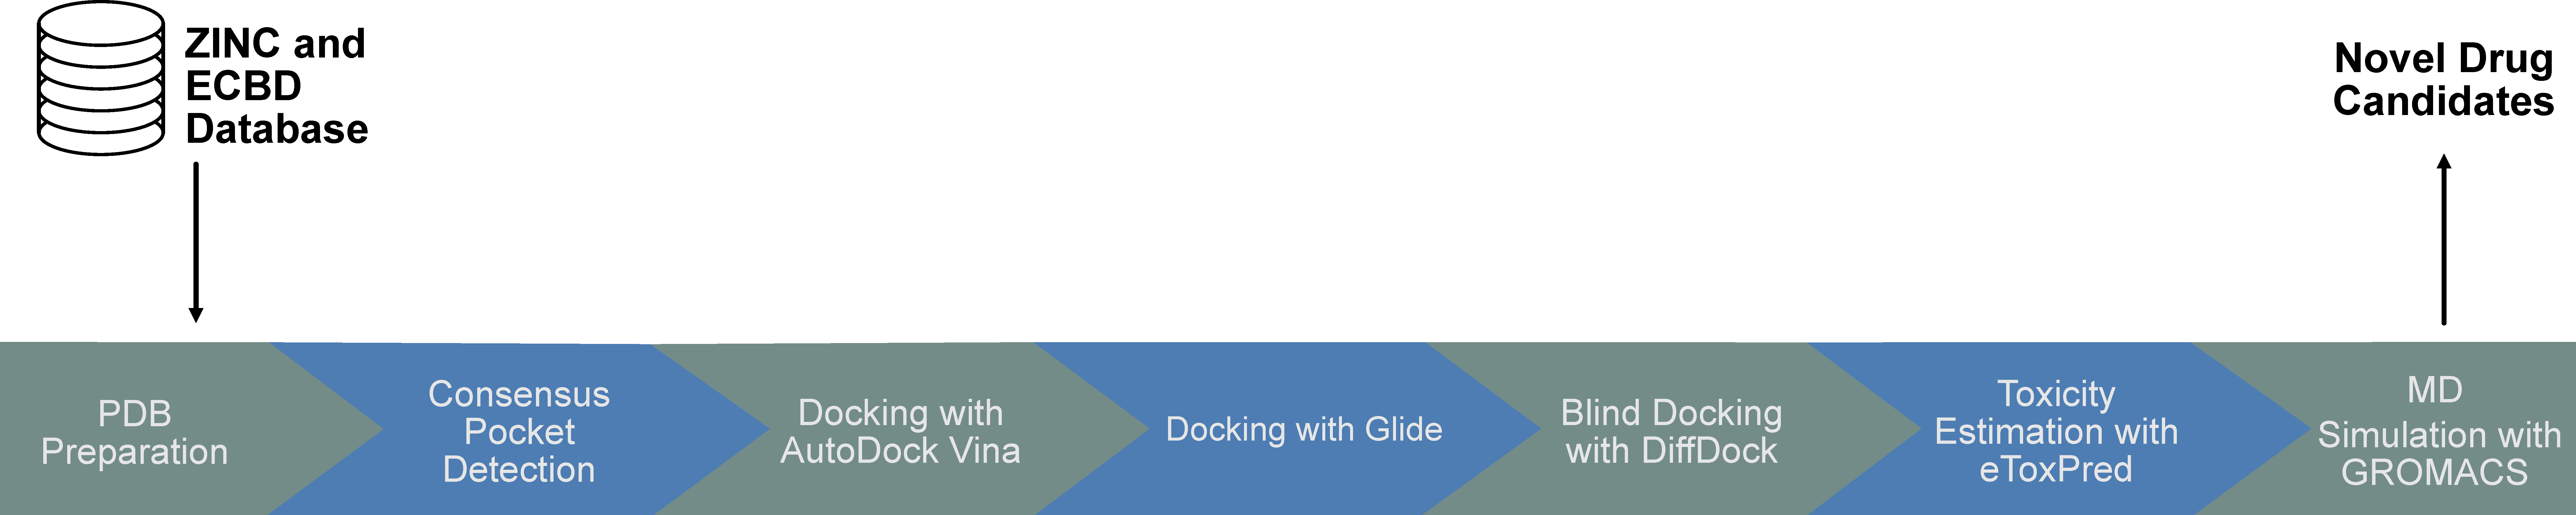
\includegraphics[width=\textwidth]{Workflow_MeetEU.pdf}
  \caption{Proposed workflow for the discovery and improvement of nsp13 helicase inhibitors.}
  \label{workflow}
\end{figure}

\FloatBarrier


\section{Introduction}
\subsection{Lead Drug Enhancement}
In order to enhance the binding affinity of our drug candidates and thus their performance, we used AutoGrow4 (Version 4.0.3) \cite{packageAutogrow4} to generate novel compounds. Starting with the best binding compounds of our initial docking simulation with AutoDock Vina as generation zero, multiple new structures are generated by combining sub-structures of the first generation or by passing them through a set of possible chemical reactions after converting them into their respective SMILES codes. All of the generated compounds are ranked by their binding affinity. After passing several filters the best performing compounds are used as the seed for the next generation. Using this algorithm, compounds are found, which show higher binding affinities than the first generation. As AutoGrow4 labels all new structures by the path by which they were obtained, we can also evaluate the synthesizability.  

\subsection{Molecular Dynamics Simulation}
As the last step of our pipeline, a MD simulation is conducted using the best scoring compounds as a ligand in the binding pocket of the NSP13 protein. Using GROMACS (Version 2023.3) \cite{packageGROMACS}, this enables us to interpret the stability of the protein-ligand interaction, as well as to identify important residues for the interaction. Using a given force-field, a set of equations describing different forces between the atoms and residues in the protein and ligand, the movement of all atoms in the system can be simulated and analysed. However, this is only possible in a very limited timeframe with a small time step size. As this process is rather resource heavy, it has to be conducted on a cluster with access to a GPU. 


\section{Material and Methods}
\subsection{Datasets from ZINC20 and ECBL}
A total of 1616 fda approved drugs were downloaded in .sdf format from the ZINC database \cite{Irwin.2020}. Additional, 5016 fiels were retrieved, downloading the pilot library from the ECBL database.

\subsection{Receptor and ligand preparation}
Ligands were prepared using openbable in order to convert implicit hydrogens into explicit hydrogens, generate necessary 3D structures of the ligands, as well as to split mulitmolecule files into single ones. ADFR suite was further used in order to convert all files into the .pdbqt format, which is required by Autodock Vina. 
 
\subsection{Generation of novel structures}
Using the same PDB file of the nsp13 A-chain, the top 10 best scoring drugs from our initial AutoDock Vina docking were passed to AutoGrow4 as SMILES. The docker container provided by the package maintainers was used, as it guarantees no problems concerning version incompatibilities. Using a similar configuration to what \Citeauthor{packageAutogrow4} used for lead drug improvement, AutoGrow4 generated and rescored a plethora of novel structures. Due to our limited amount of structures in generation zero, we opted to disable the generation of cross-over molecules for the first generation. The configuration file can be found in the appendix. As we try to improve a small amount of lead drugs, AutoGrow4 generates many new molecules per generation, while it is only run for five generations. This enables us to explore different modifications to our compounds while not making synthesis too complicated, as there is a maximum of five modifications happening. Because AutoGrow4 also enables structures with a diverese structure to pass into next generations even though they might not be top performers yet, we can be sure to explore a vast landscape of different possible drugs.

\subsection{Molecular Dynamics Simulation}
In order to validate the binding of the discovered compounds, we used GROMACS to simulate the drugs inside of the ATP binding site of nsp13. To do so, the Protein-Ligand Complex tutorial by \Citeauthor{Lemkul2018} was used \cite{Lemkul2018}. The a99SB-disp forcefield was used, as it was shown to recreate protein structures in different environments very accurately \cite{Forcefield}. 
\section{Results} 

\FloatBarrier

\section{Discussion and Outlook}

\section{Supplementary Material}

\pagebreak
\FloatBarrier

\renewcommand{\bibname}{References}  % damit Literatuverzeicnis mit "References" betitelt
\printbibliography


\end{document}
